\chapter{Thrust 1: Stakeholder Engagement}\label{chap:thrust1}

One of the aims of this project was to make fuel cycle simulation and analysis
accessible to a broader audience of users by designing different user
experiences for different categories of users.  Doing so requires that the
interests and use cases of those different categories be sufficiently
understood.  The overarching goal of Thrust 1 was to determine the
specific kind of information that various users and stakeholders would like to
learn from a nuclear fuel cycle simulator to support their application of such
a tool.  This thrust was born from a recognition that different categories of
users would be interested in different kinds of information, possibly
different from the set of information traditionally provided by the fuel cycle
experts who typically study such systems.  Moreover, the fidelity and nuance
surrounding that information may vary across groups of users.

One of the innovative aspects of this project was the incorporation of social
science research as a full partner.  This thrust was led by Prof. Dominique
Brossard of the Life Science Communication Department at the University of
Wisconsin-Madison.  This thrust incorporated established methods of social
science research to study both the kind of information that users would be
interested in learning, as well as the impact of different visualization modes
on their understanding of that information.  More details about the studies
described in this chapter can be found in the PhD dissertation of Dr. Nan Li
\citeprod{li-dissertation}.

The first task in this thrust was to identify different communities of
stakeholders and the issues that are most important to those communities.
Informed, in part, by this information, the second task assessed how different
aspects of a data visualization affected the integration of that data by
different stakeholder audiences.

\section{Stakeholder and Issue Identification}

This task followed a well-established social science research protocol for
identifying and characterizing stakeholder groups and their most important
issues, beginning with a thorough review of documents related to nuclear fuel
cycles, continuing with a round of qualitative research in which a set of
stakeholders was interviewed, and concluding with quantitative research in the
form of a survey of a larger set of those stakeholders.

Because the \gls{ngfcs} was not sufficiently advanced at the beginning of the
research project to support a wide variety of stakeholders, the scope of this
thrust was narrowed to focus on federal decision makers: Congressional staff,
employees of federal agencies, and national think-tanks and non-profits.

\subsection{Document Review \& Analysis}

The starting point of this research was to collect and review a wide array of
publicly available documents related to public policy and public engagement
around the nuclear fuel cycle.  These documents came from many sources, with a
large fraction coming from public testimony before various panels and
committees.  The most recent set of documents, for example, came from
testimony and contributions to the Blue Ribbon Commission on America's Nuclear
Future, that had concluded its review just as this project began.

This kind of review is a critical step for establishing first a fundamental
knowledge of the vocabulary and terminology, and then using that to identify
the different categories of stakeholders.  For each category of stakeholder,
this analysis also helped to identify the important issues when they consider
existing or potential future nuclear fuel cycles.  The primary outcome of
this phase was the development of an list of potential interviewees and a
script to conduct those interviews.

\subsection{Stakeholder Interviews}

Interviews were were conducted with 12 individuals from the nuclear energy
policy community, with two purposes.  Individuals were identified by reviewing
all the public hearing records found by searching for ``nuclear'' in the
ProQuest Congressional Publications database between May 2009 and March 2012.
From these documents spanning topics from waste management to profliferation
to safety, a cohort of policy experts with varying professional backgrounds,
experiences and interests was recruited.


First, the content of these interviews would provide a more nuanced
understanding of the issues identified in the document review in order to
formulate survey questions for a larger sample.  Figures \ref{fig:interview_1}
and \ref{fig:interview_2} show the issue categories identified through this
process for nuclear energy in general and advanced fuel cycles in specific.
Interviewees were also solicited for specific recommendations of information
that a \gls{nfcs} might be able to provide to help inform their understanding
and decision making around nuclear fuel cycles.  These specific
recommendations were allocated to seven categories:
\begin{enumerate}
\item General,
\item Environmental and Health Safety,
\item Waste Management,
\item Cost and Economic Issues,
\item Resource Utilization,
\item Sustainability, and
\item Non-proliferation.
\end{enumerate}

Each category contained at least seven (Sustainability) and up to 38 (Cost and
Economic Issues) specific recommendations.  Two categories (Environmental and
Health Safety and Cost and Economic Issues) had six recommendations that were
mentioned by more than one interviewee.

\begin{figure}[htbp]
  \centering
  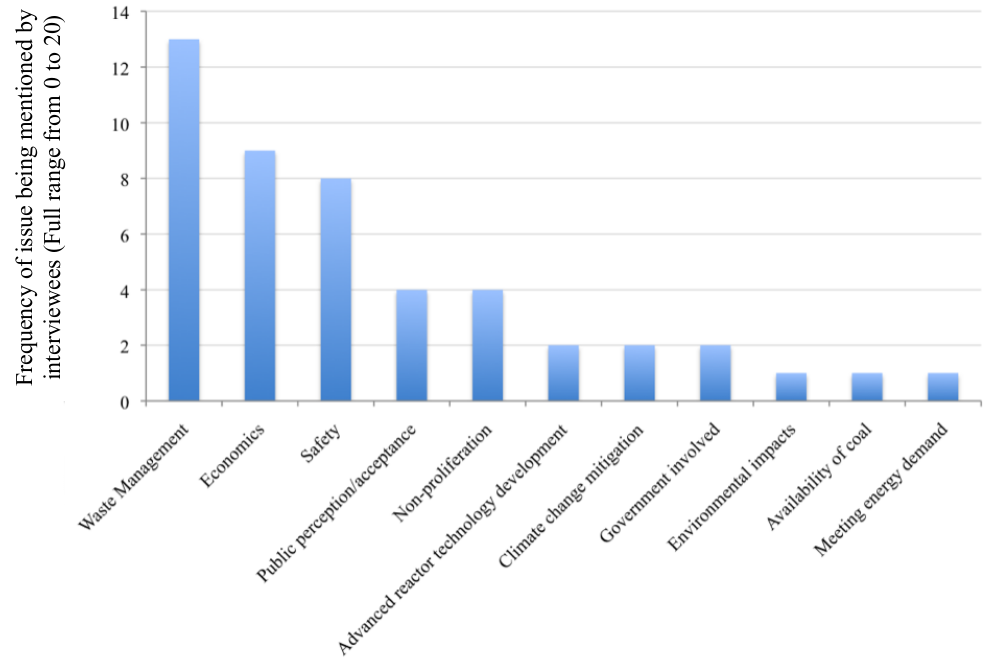
\includegraphics[width=0.7\columnwidth]{./images/interview_1}
  \caption{Main Issues Related to Nuclear Energy Identified Through Qualitative Interviews}
  \label{fig:interview_1}
\end{figure}

\begin{figure}[htbp]
  \centering
  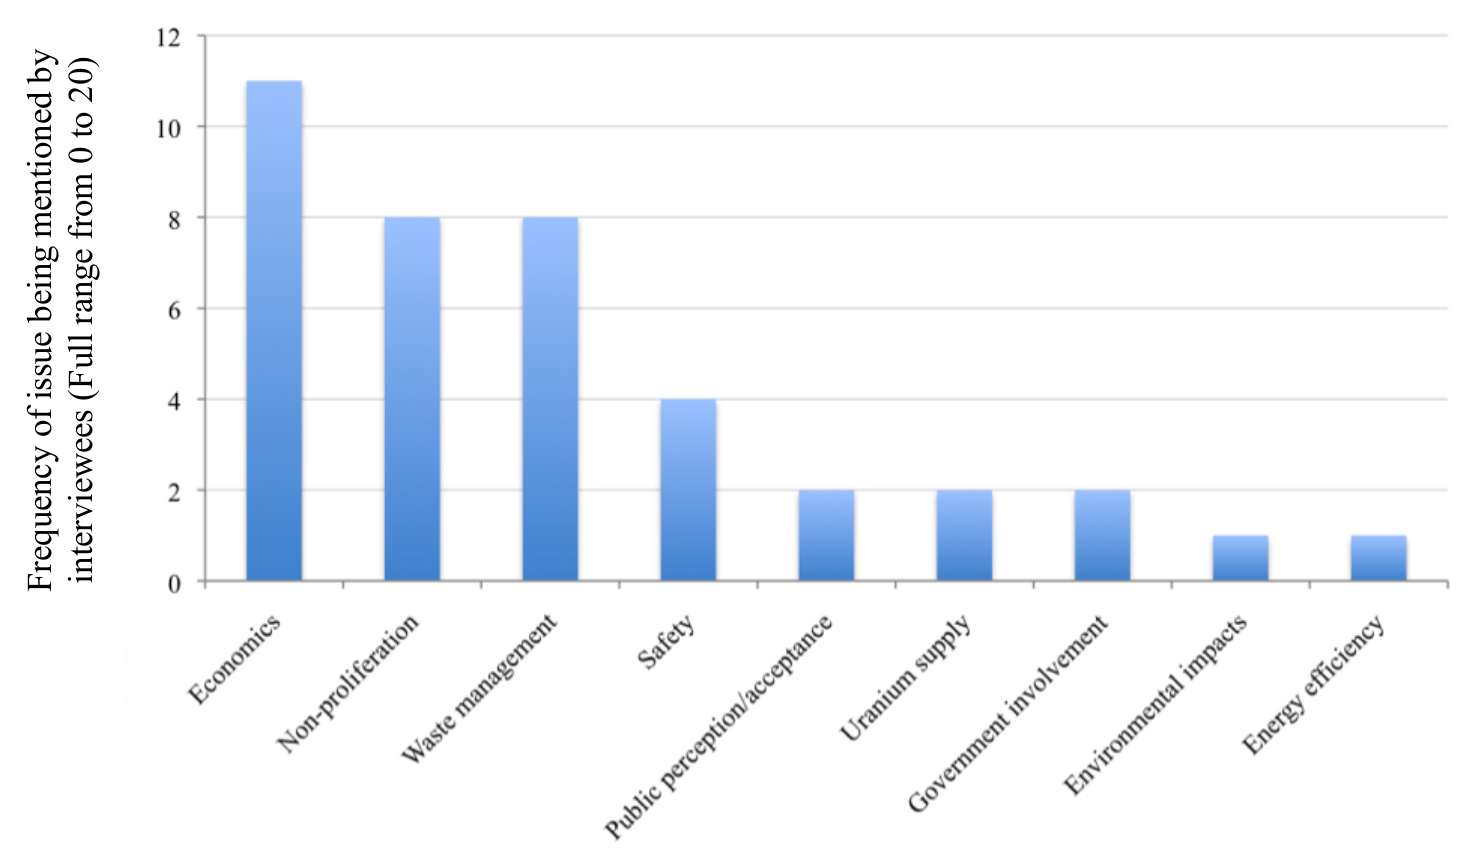
\includegraphics[width=0.7\columnwidth]{./images/interview_2}
  \caption{Main Issues Related to Advanced Fuel Cycles Identified Through Qualitative Interviews}
  \label{fig:interview_2}
\end{figure}

The second purpose of these interviews was to perform semantic computational
analysis of the language in the transcripts of those interviews.  The CATPAC
II software was used to detect patterns and correlations between different
conceptual words that appear in the transcripts by recording their frequency
of occurring together in a moving 5 word window.  The fundamental measures of
connection between concepts can be analyzed with a number of techniques,
including a multidimensional scaling (MDS) analysis.  The MDS analysis results
can be visualized in a 2D or 3D space to identify emergent meanings and
dominant themes.  Figure \ref{fig:word_frequency_mds} shows such a
visualization for the terms identified in the transcripts of the six
interviews conducted with government policymakers.

\begin{figure}[htbp]
  \centering
  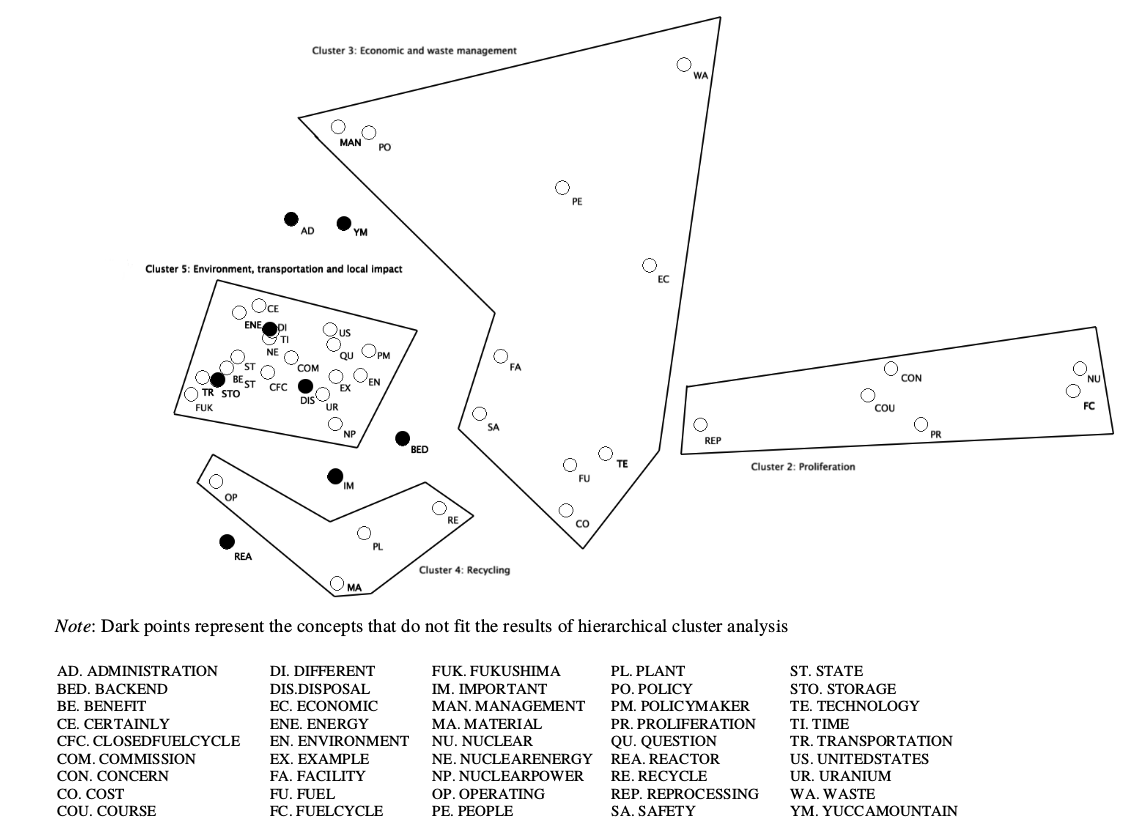
\includegraphics[width=0.7\columnwidth]{./images/word_frequency_mds}
  \caption{2D Representation of Unique Concepts for Government Policymaker Interviewees.}
  \label{fig:word_frequency_mds}
\end{figure}

A similar analysis for the six interviews conducted with non-profit/think-tank
experts showed that different clusters emerge, suggesting nuanced differences
in how policymakers and think-tank experts characterize the most important
issues facing the development of the nuclear fuel cycle.

\subsection{Stakeholder Survey}

A survey was constructed with seven questions specifically related to nuclear
energy, advanced fuel cycles, and \glspl{nfcs}, followed by three questions
that assess the respondents' beliefs on the relationships between science, the
media and policy, and five demographic questions (see Appendix
B of Ref \citeprod{li-dissertation}).  Two central questions asked respondents about possible
output metrics from a \gls{nfcs}, specifically asking them to judge both the
importance of the metric and the level of confidence with which they believed
that metric could be calculated.

The survey was sent to 557 policy stakeholders including:
\begin{enumerate}
\item 404 attendees of the public hearings documented above, 
\item 63 former members of Congress or their staff that focused on energy issues determined from reviewing the directories of the 109$^{th}$ through 111$^{th}$ Congress, and
\item 90 state and local stakeholders determined by reviewing the public
  meetings held by the Blue Ribbon Commisison for America's Nuclear Future in
  2011.
\end{enumerate}
After a number of rounds of reminders, a total of 137 completed surveys
(27.4\% response rate) were returned and analyzed.

One type of analysis sought to test a hypothesis identified in the interview
analysis that the institutional identity of a respondent would influence their
perception of the importance of different issues, as well as their view of the
role of science as a driver of policy.  This analysis found that industry and
advocacy groups were less likely to think that environmental health and safety
should be taken into account when developing advanced nuclear fuel cycles,
whereas academic stakeholders were less likely to consider nuclear waste
management as an important issue for advanced fuel cycle development.

One of the important results of the survey was to sort the issues related to
advanced nuclear fuel cycles by their perceived importance as metrics for a
\gls{nfcs} and by the perceived confidence in being able to calculate such
metrics.  Of the thirteen issues that were ranked with high importance, five
of them were also ranked with high confidence while the remaining eight were
ranked with low confidence.

\begin{itemize}
\item \textbf{High Importance, High Confidence}:
  \begin{itemize}
  \item fuel types and reactor types needed
  \item long-term nature of nuclear fuel cycle
  \item impact of nuclear fuel cycle on energy generation
  \item waste volumes
  \item waste types
  \end{itemize}
\item \textbf{High Importance, Low Confidence}:
  \begin{itemize}
  \item operating costs
  \item costs of entire nuclear fuel cycle
  \item cost of waste disposal space
  \item amount of sustained funding
  \item probability of accidental release
  \item impacts on local economies
  \item attractiveness to utility companies
  \item public acceptance
  \end{itemize}
\item \textbf{Low Importance, High Confidence}:
  \begin{itemize}
  \item amount of uranium needed
  \item amount of mining
  \end{itemize}
\item \textbf{Low Importance, Low Confidence}:
  \begin{itemize}
  \item availability of uranium resource
  \item cost of building public support
  \item carbon price
  \end{itemize}
\end{itemize}

The most important issues should be identified as priorities for
implementation in a \gls{ngfcs} and those that are also deemed low confidence
should bre identified as research priorities in an effort to reduce their
uncertainty and raise confidence in being able to present such metrics.

\section{Assessing Visualization Efficacy and Credibility} %% Sci Comm paper

The second major component of Thrust 1 was to assess the effectiveness of
different visualization modes for communicating information from a \gls{nfcs}.
Because the \Cyclus simulator was not sufficiently advanced, a surrogate set
of visualizations was used for testing.  Because both were indicated as
important in the prior work, the visualization testing used mock data for
costs and waste management.  Experiments were constructed in which a
respondent was shown a visualization of this data and asked to respond to a
set of questions regarding both the data itself and the visualization that was
used to communicate the data.

A total of 517 valid responses to the experiment were collected from
undergraduate students at the University of Wisconsin-Madison from a variety
of disciplines and backgrounds.  They were divided roughly evenly between
science \& engineering (28.7\%), social sciences (32.9\%), and the humanities
(31.9\%), and were almost all (98\%) between the ages of 18-24.  The majority
(64\%) were females and about the same fraction were either freshman or
sophomores.

In each case, the respondents were first asked a series of questions about
themselves, designed to probe the following:
\begin{itemize}
\item familiarity with nuclear energy issues
\item perceived credibility of different information sources
\item self-assessment of numeracy and graph literacy
\end{itemize}

Each respondent was then shown one visualization of mock data related to
nuclear fuel cycles.  A number of characteristics of the visualizations were
varied across the sample of respondents:
\begin{itemize}
\item area chart vs bubble chart
\item static chart vs interactive chart
\item cost vs mass
\item government attribution vs academic attribution
\end{itemize}
Figures \ref{fig:viz-area-static-cost} and \ref{fig:viz-bubble-dynamic-waste}
show two of the sixteen possible combinations.

\begin{figure}[htbp]
  \centering
  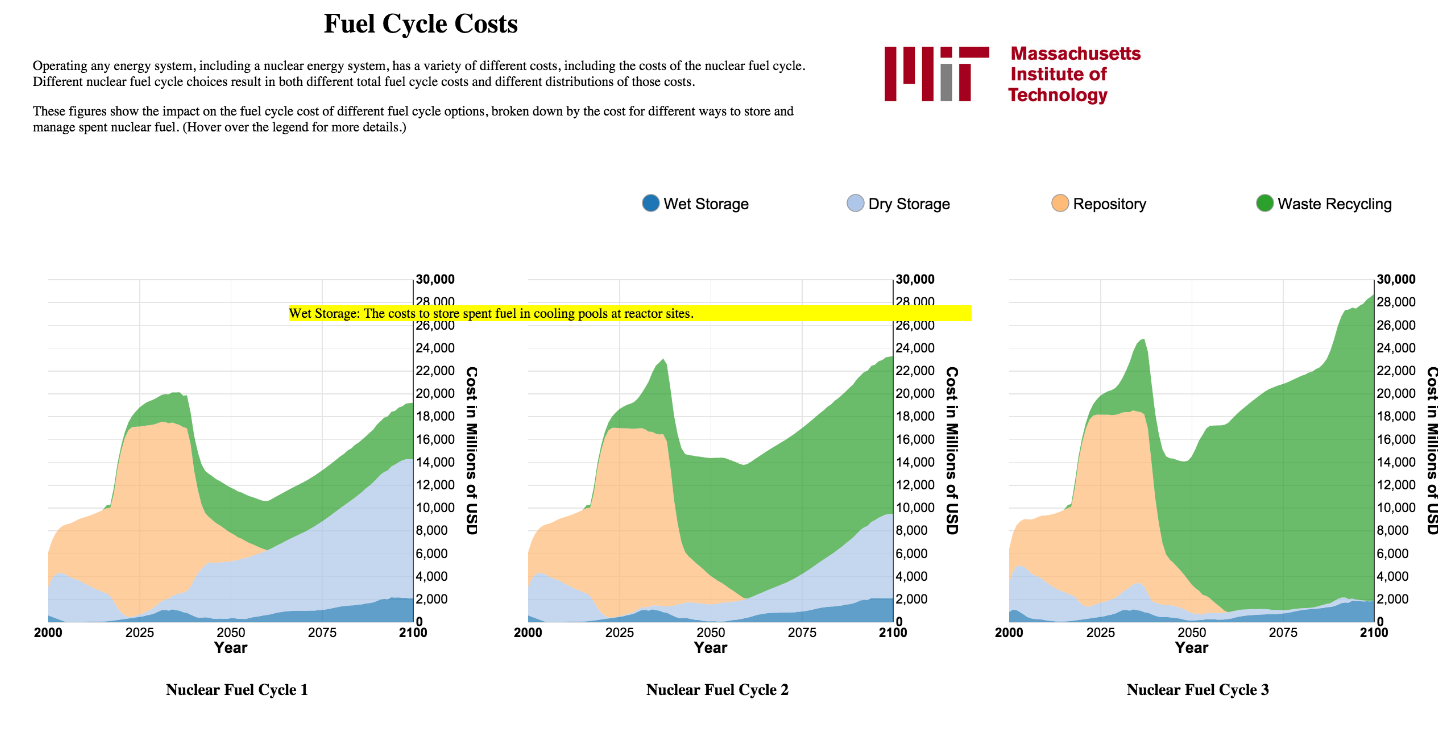
\includegraphics[width=\columnwidth]{./images/viz-area-static-cost}
  \caption{Static area chart depicting fuel cycle costs for three different
    options over time.  The interactive version allowed the viewer to query the
    values at any year.}
  \label{fig:viz-area-static-cost}
\end{figure}

\begin{figure}[htbp]
  \centering
  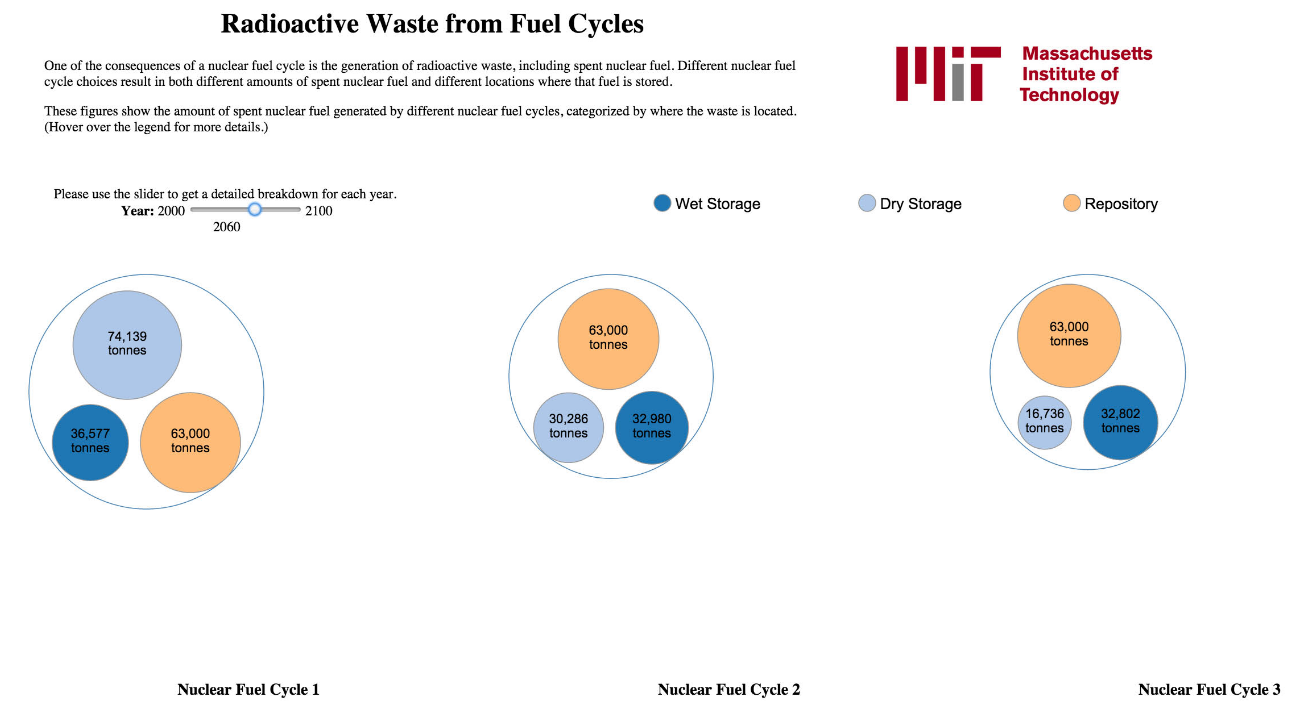
\includegraphics[width=\columnwidth]{./images/viz-bubble-dynamic-waste}
  \caption{Interactive bubble chart depicting the mass of waste for three
    different options over time.  The slider in this version allowed the viewer
    to see the mass of waste at different years.  The static version showed
    only three specific years for each case.}
  \label{fig:viz-bubble-dynamic-waste}
\end{figure}

After viewing one of the sixteen possible variations, respondents were asked a
series of questions about the data they had seen.  Some questions tested how
accurately the respondents could interpret the data, both in absolute terms by
asking for specific values, and in relative terms by asking for comparisons.
Related questions tested the quality of decision making by asking respondents
to identify the best option given particular goals.  Other questions tested
the opinions of the respondents with regards to the perceived credibility and
the perceived effectiveness of the visualization.

Finally, a set of questions was used to further probe the numeracy of the
respondent, both in terms of their self reported perceived numeracy and by
asking a series of questions about unrelated data.

\subsection{Graph Comprehension}

Statistical regression analysis was used to determine the contribution of each
control variable in explaning the observed variance in graph comprehension, as
measured by the respondents ability to indicate quantitative results from the
visualized data.  The biggest contributor to comprehension was the format of
the visualization, with respondents performing better when viewing the bubble
chart.  The next largest contributor was the interactivity of the
visualization, with respondents performing better when they viewed an
interactive graph, although only for the area charts.  While general graph
literacy was positively correlated to comprehension, specific domain knowledge
did not have an impact.

\subsection{Decision Quality}

Another regression analysis was used to determine the quality of decisions
made by respondents, as measured by their ability to identify the best option
from among three fuel cycles.  Despite the indications that respondents had a
better quantitative understanding of bubble charts over area charts, those
respondents who viewed area charts were better able to select the option that
correpsonded to the requested optimum.  Numeracy skills and graph literacy
also resulted in better likelihood of success in identifying an optimum.

\subsection{Credibility}

The final analysis considered the perceived credibility of the data shown in
the visualizations\citeprod{li_credibility}.  The perceived credibility was
not impacted by the format of the chart, although respondents did perceive the
static charts are slightly more credible than the interactive charts.  The
visualizations attributed to an academic source were perceived as more
credible overall.  This was mediated by the respondents' predisposition to
trust academic sources relative to governmental sources.  Those respondents
who reported a higher trust for academic sources perceived more credibility in
the data attributed to an academic source, while those respondents who
reported a higher trust for governmental sources did \emph{not} perceive more
credibility in the data attributed to a government source.  Overall, younger
respondents were more skeptical of the data.  Regarding the visualization
itself, the respondents' evaluation of the quality of the visualization, and
their own ability to read and use graphical tools in general, were more
important for supporting credibility than their measured comprehension of the
data.


\section{Summary}

A rigorous social science study of the issues surrounding nuclear fuel cycles
was carried out to understand the role of a \gls{nfcs} in decision making.
While a number of stakeholder groups were identified, the bulk of the study
focused on federal decision makers and think tank experts.  A combination of
document review and a dozen interviews were used to identify a set of issues
that formed the basis of a survey instrument that was sent to 517 individuals,
receiving 137 responses.  A principal outcome of the survey was to identify
which issues that had been raised earlier were considered important for a
\gls{nfcs}, and separately, which issues the respondents believed could be
credibly produced by a \gls{nfcs}.  Two metrics that represented the important
issues were used to create a visualization experiment in order to study how
different aspects of the visualization impacted the comprehension of the data,
the quality of decision making based on that data, and the credibility of the
information.  While this last step did not use \Cyclus visualizations
directly, it did provide information about the future direction of
visualization of \gls{nfcs} results.
